\chapter{Vizualizácie}
\epigraph{An algorithm must be seen to~be~believed.}{\textit{The Art of Computer Programming}\\ \textsc{Donald E. Knuth}}

Cieľom tejto práce je nielen popísať \obliv pamäťový model a rôzne dátové štruktúry v ňom, ale aj vytvoriť ich vizualizácie. Tie majú slúžiť na edukačné účely pre študentov (a učiteľov) a pomáhať pri pochopení ich fungovania.

Výsledkom práce sú vizualizácie demonštrujúce dátové štruktúry popísané v predchádzajúcich sekciách: \vEB usporiadanie (sekcia \ref{sec:static-obliv}) v statickom binárnom vyhľadávacom strome, usporiadané pole (\ref{sec:orderedfile}) a dynamický B-strom (\ref{sec:dynamic-obliv}). Súčasťou je tiež simulácia \cache (sekcia \ref{sec:extmem}) s možnosťou voľby parametrov $B$ a $M$ - veľkosť bloku a celková veľkosť.

\todo[inline]{Existujuce? nic nie je...}

\section{Gnarley trees}
Tieto vizualizácie sú implementované ako rozšírenie programu \emph{Gnarley trees}, ktorý vznikol ako súčasť bakalárskej práca Jakuba Kováča \citep{algviskuko}. Tento nástroj na vizualizáciu (prevažne stromových) dátových štruktúr bol následne v bakalárskych prácach \citep{algviskotrlova, algvistomkovic, algvislukca} a ročníkových projektoch rozšírený o mnohé ďalšie dátové štruktúry a v súčastnosti podporuje desiatky štruktúr, ako napríklad červeno-čierne, sufixové a intervalové stromy, \emph{union-find}, haldy a mnohé ďalšie.

\subsection{Spustenie}
Súčasťou práce je priložené CD obsahujúce zdrojový kód tohto programu a tiež skompilovanú verziu. Aplikácia na spustenie požaduje \emph{JVM}\footnote{\emph{Java Virtual Machine}, dostupné na \url{https://www.java.com/en/download/}}. Spustenie je možné vykonať spustením súborov \inlcode{start.sh} prípadne \inlcode{start.bat}, podla operačného systému. Dostupné sú tiež individuálne vizualizácie vo forme \emph{Java appletov}, ktoré je možné spustiť otvorením súboru \inlcode{index.html} v preferovanom internetovom prehliadači.

Obsah tejto CD prílohy je tiež dostupný na \todo{url}.

\subsection{Funkcionalita}
Program umožňuje užívateľom zobrazovať tieto štruktúry a manipulovať s nimi. Všetky operácie sú rozložené na malé, jednoduché kroky a každý je vysvetlený, keď sa vykonáva. Je možné posúvať sa po krokoch dopredu, ale aj vracať sa dozadu, a teda sa dá kedykoľvek vrátiť až k počiatočnému stavu. Toto je dôležité pri experimentovaní s danou štruktúrou, kedy dve rôzne operácie (alebo jedna operácia s dvoma rôznymi parametrami) spôsobia rôzne správanie a výsledky. Užívateľ má takto možnosť jednoducho sa po vykonaní prvej operácie vrátiť do predošlého stavu a preskúmať správanie druhej z nich.

Celý program je taktiež dvojjazyčný - je možné prepnúť medzi angličtinou a slovenčinou, čo umožňuje širšie použitie týchto vizualizácií.

\subsection{Prehľad programu}
\begin{figure}
    \centering
    \resizebox{0.9\textwidth}{!}{%
        \begin{tikzpicture}

\node[anchor=south west,inner sep=0] (IMG) at (0,0) {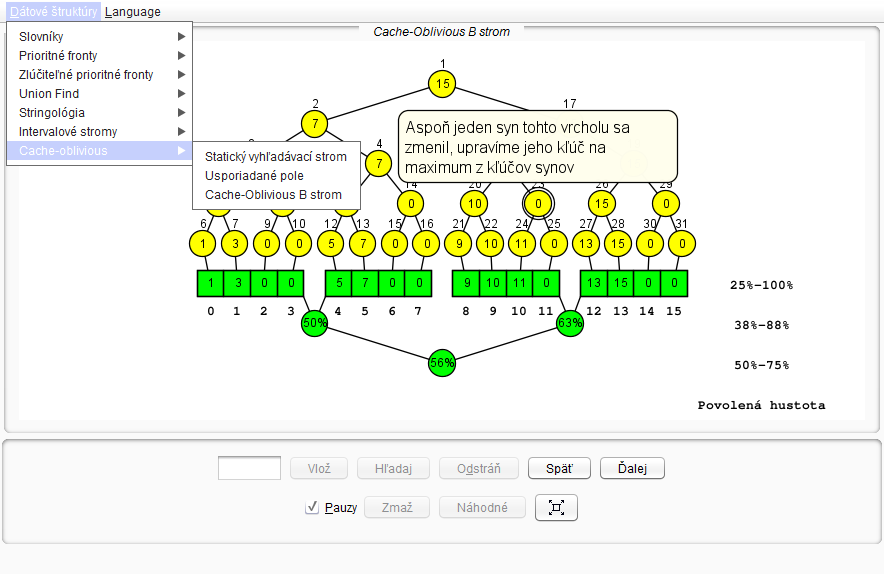
\includegraphics[width=18cm]{\FiguresPath/screenshots/bmp_cobtree_menu_sk}};
\draw [thick, darkgray] (IMG.south west) rectangle (IMG.north east);

%\draw[draw=red,xstep=1,ystep=1] (0,0) grid (18,12);
%\foreach \x in {0,1,...,18} { \node [anchor=north] at (\x,0) {\x}; }
%\foreach \y in {0,1,...,12} { \node [anchor=east] at (0,\y) {\y}; }

\draw [thick, ->] (2, 12.5) node [anchor=west] {Výber dátovej štruktúry} to [in=90, out=180] (1, 11.75);
\draw [thick, ->] (3, 12) node [anchor=west] {Výber jazyka} to [in=90, out=180] (2.5, 11.75);

\draw [thick, ->] (10, 12.5) node [anchor=west] {Aktuálna dátová štruktúra} to [in=90, out=180] (9, 11.25);

\draw [thick, ->] (13, 12) node [anchor=west] {Popis vykonávanej akcie} to [in=90, out=180] (11, 9.5);

\draw [thick, decoration={brace, amplitude=10pt, 
	/tikz/postaction = {
		decoration = {
			markings,
			mark = at position 0.5 with \coordinate (CP);
		}, decorate
	}
}, decorate] (4.25, 1) -- (4.25, 2.5);
\draw [thick] (2.5, -0.5) node [anchor=east] {Ovládací panel} to [in=180, out=0](CP);

\draw [thick, ->] (7, -0.5) node [anchor=west] {Povolenie krokovania} to [in=270, out=180] (6.35, 1.15);

\draw [thick, decoration={brace, amplitude=10pt, mirror,
	/tikz/postaction = {
		decoration = {
			markings,
			mark = at position 0.5 with \coordinate (PN);
		}, decorate
	}
}, decorate] (10.65, 1.95) -- (13.7, 1.95);
\draw [thick] (13, -0.5) node [anchor=west] {Krokovanie dopredu / dozadu} to [in=270, out=180] (PN);

\end{tikzpicture}    
    }
    \caption[Užívateľské rozhranie]{Užívateľské rozhranie počas operácie vkladania kľúča $10$ do dynamického \obliv B-stromu (sekcia \ref{sec:dynamic-obliv}).}
    \label{fig:ss_overview}
\end{figure}

Program sa skladá z troch hlavných častí (obrázok \ref{fig:ss_overview}). Najvrchnejšia časť okna tvorí hlavné menu, v ktorej môžeme voliť dátové štruktúry a prepínať jazyk rozhrania. Dátové štruktúry sú pre prehľadnosť rozdelené do niekoľkých kategórií. Tie popísané a implementované v tejto práci sa nachádzajú v kategórii \texttt{Cache-oblivious}.

V spodnej časti okna sa nachádza ovládací panel, ktorý obsahuje vstupné pole pre hodnotu, ktorú chceme vyhľadať alebo vložiť a tlačidlá na vykonanie týchto akcií. Ďalej obsahuje tlačidlá na prechod do ďalšieho kroku a návrat do predchádzajúceho stavu s možnosťou toto krokovanie vypnúť.

Najväčšia, prostredná časť okna zobrazuje vizualizáciu aktuálnej dátovej štruktúry. Toto zobrazenie je vektorové a je možné ho posúvať, približovať a oddaľovať. Zároveň sa tu zobrazujú informácie o aktuálne vykonávanej akcií (ak je povolené krokovanie) a ďalšie vizualizačné prvky ako šípky alebo význačné vrcholy.

Podrobnejší popis užívateľského rozhrania a návod na používanie sa nachádza v bakalárskej práci Jakuba Kováča \citep{algviskuko} v siedmej kapitole.

\section{Statický strom}
Najjednoduchšou dátovou štruktúrou je statický vyhľadávací strom. Implementovali sme vytvorenie tohto stromu a jeho uloženie v pamäti. Je možné strom zväčšiť alebo zmenšiť podľa preferencii - ukážky stromov rôznych veľkostí sú na obrázku \ref{fig:ss_static_sizes}. Čísla vo vnútorných vrcholoch sú kľúče, čísla nad vrcholom určujú jeho pozíciu v pamäti. Obdĺžnik nad stromom reprezentuje uloženie tohto stromu v poli. Vnútorné čísla sú opäť kľúče, pričom sú zoradené podľa svojich pozícii zľava (pozícia $1$) doprava.

\begin{figure}
    \centering
    \subtop[]{%
        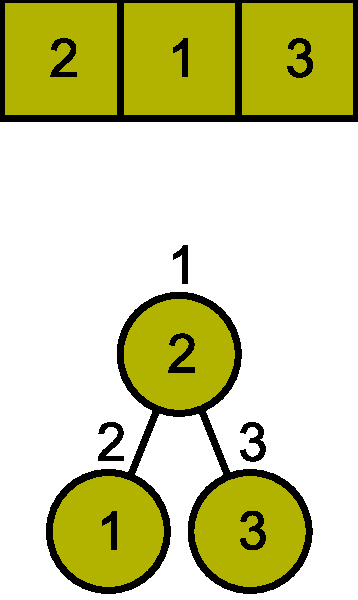
\includegraphics[scale=0.25]{figures/screenshots/static_size_2.pdf}}
    \hspace{0.5cm}
    \subtop[]{%
        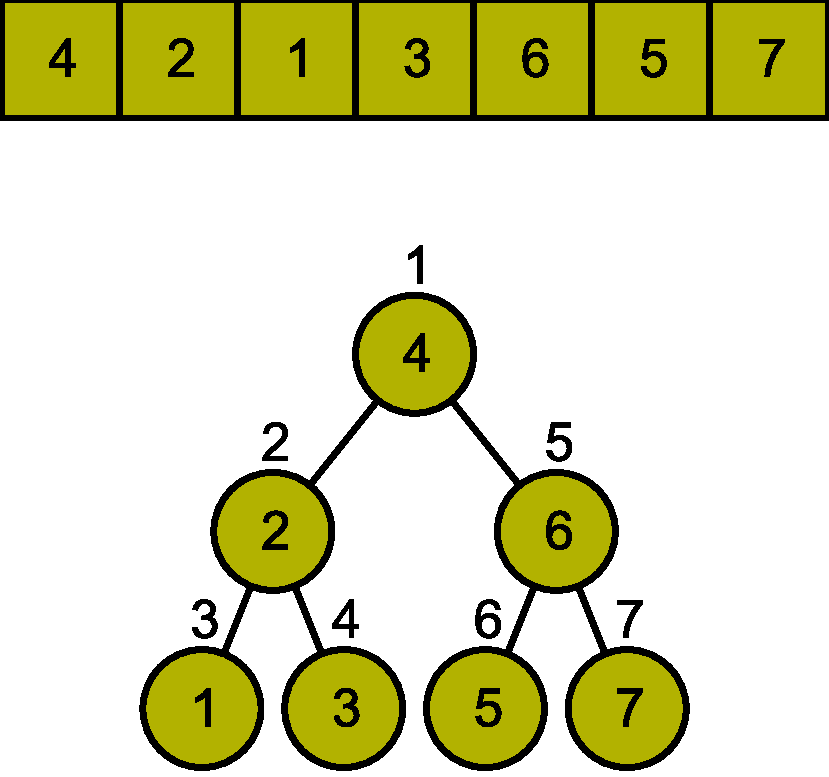
\includegraphics[scale=0.25]{figures/screenshots/static_size_3.pdf}}
    \hspace{0.5cm}
    \subtop[]{%
        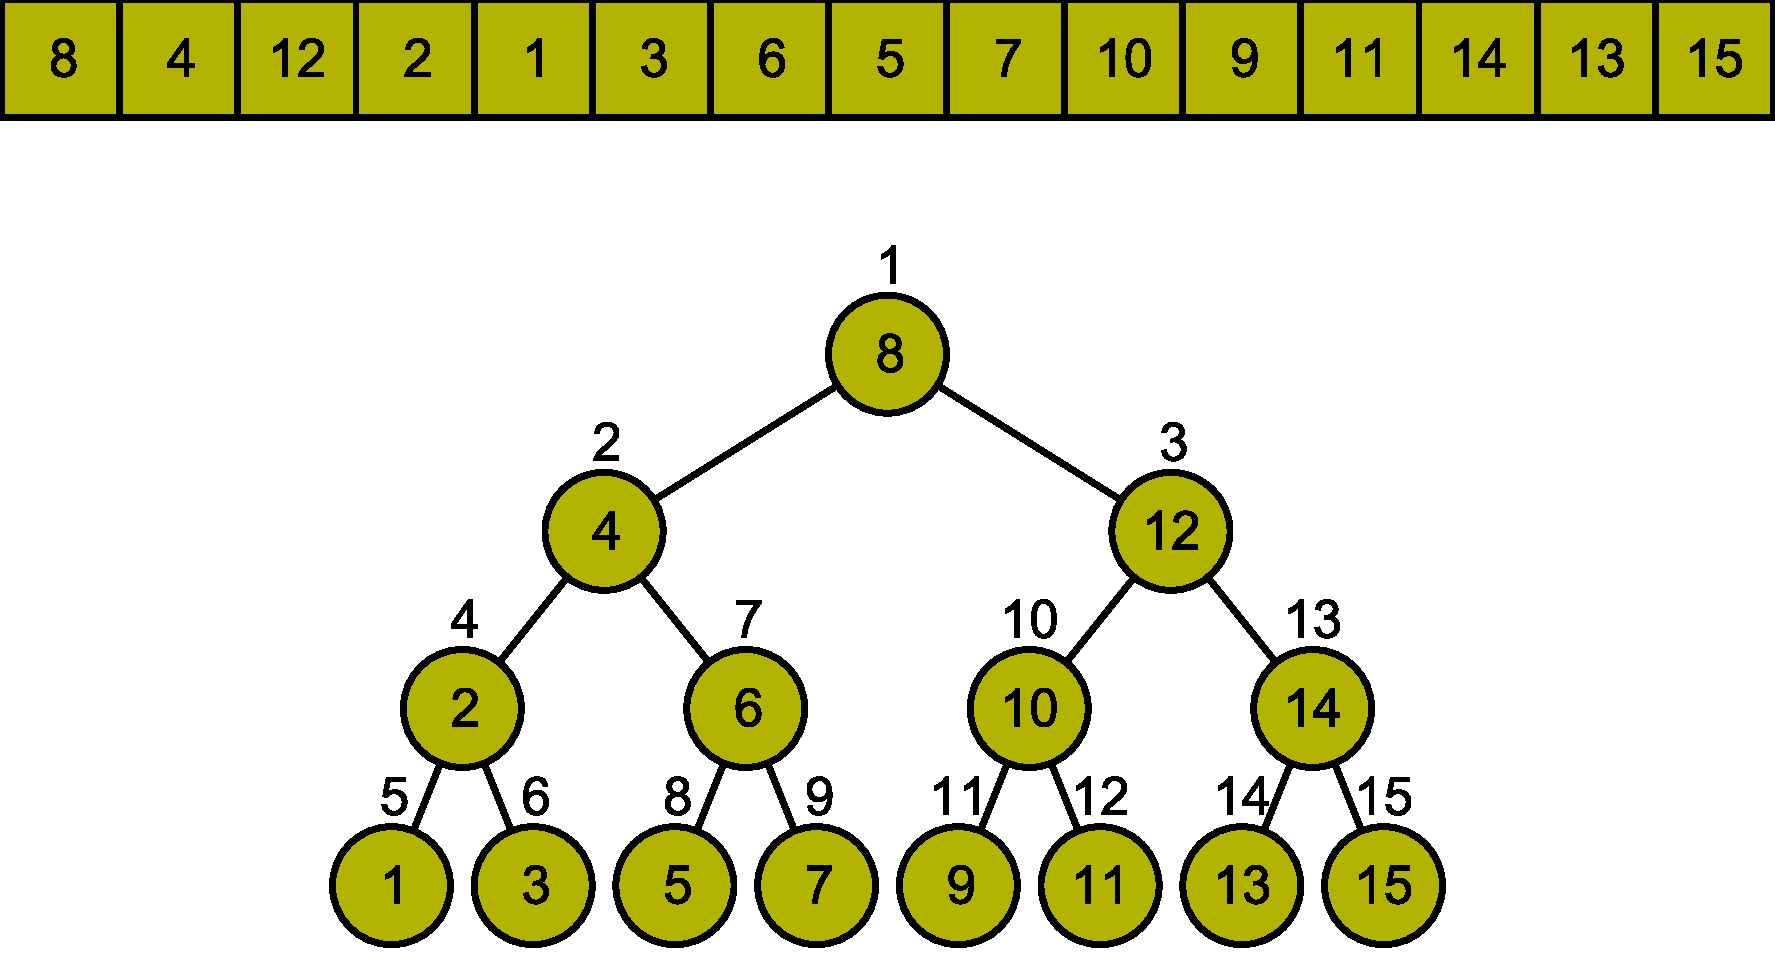
\includegraphics[scale=0.25]{figures/screenshots/static_size_4.pdf}}
    \caption[Statické stromy rôznych veľkostí]{Statické stromy rôznych veľkostí (výšok) vo \vEB usporiadaní.}
    \label{fig:ss_static_sizes}
\end{figure}

Medzi uložením vo \vEB usporiadaní a klasickom \emph{BFS} usporiadaní (ako v časti \ref{sec:static-naive}) je možné prepínať. Zmenia sa pritom čísla udávajúce pozície vrcholov v pamäti a ich poradie v poli nad stromom. Rozdiel medzi týmito dvoma usporiadaniami vidieť na obrázku \ref{fig:ss_static_order}. Pozície sa zhodujú s obrázkom \ref{fig:node_order_veb}.

\begin{figure}
    \centering
    \subtop[]{%
        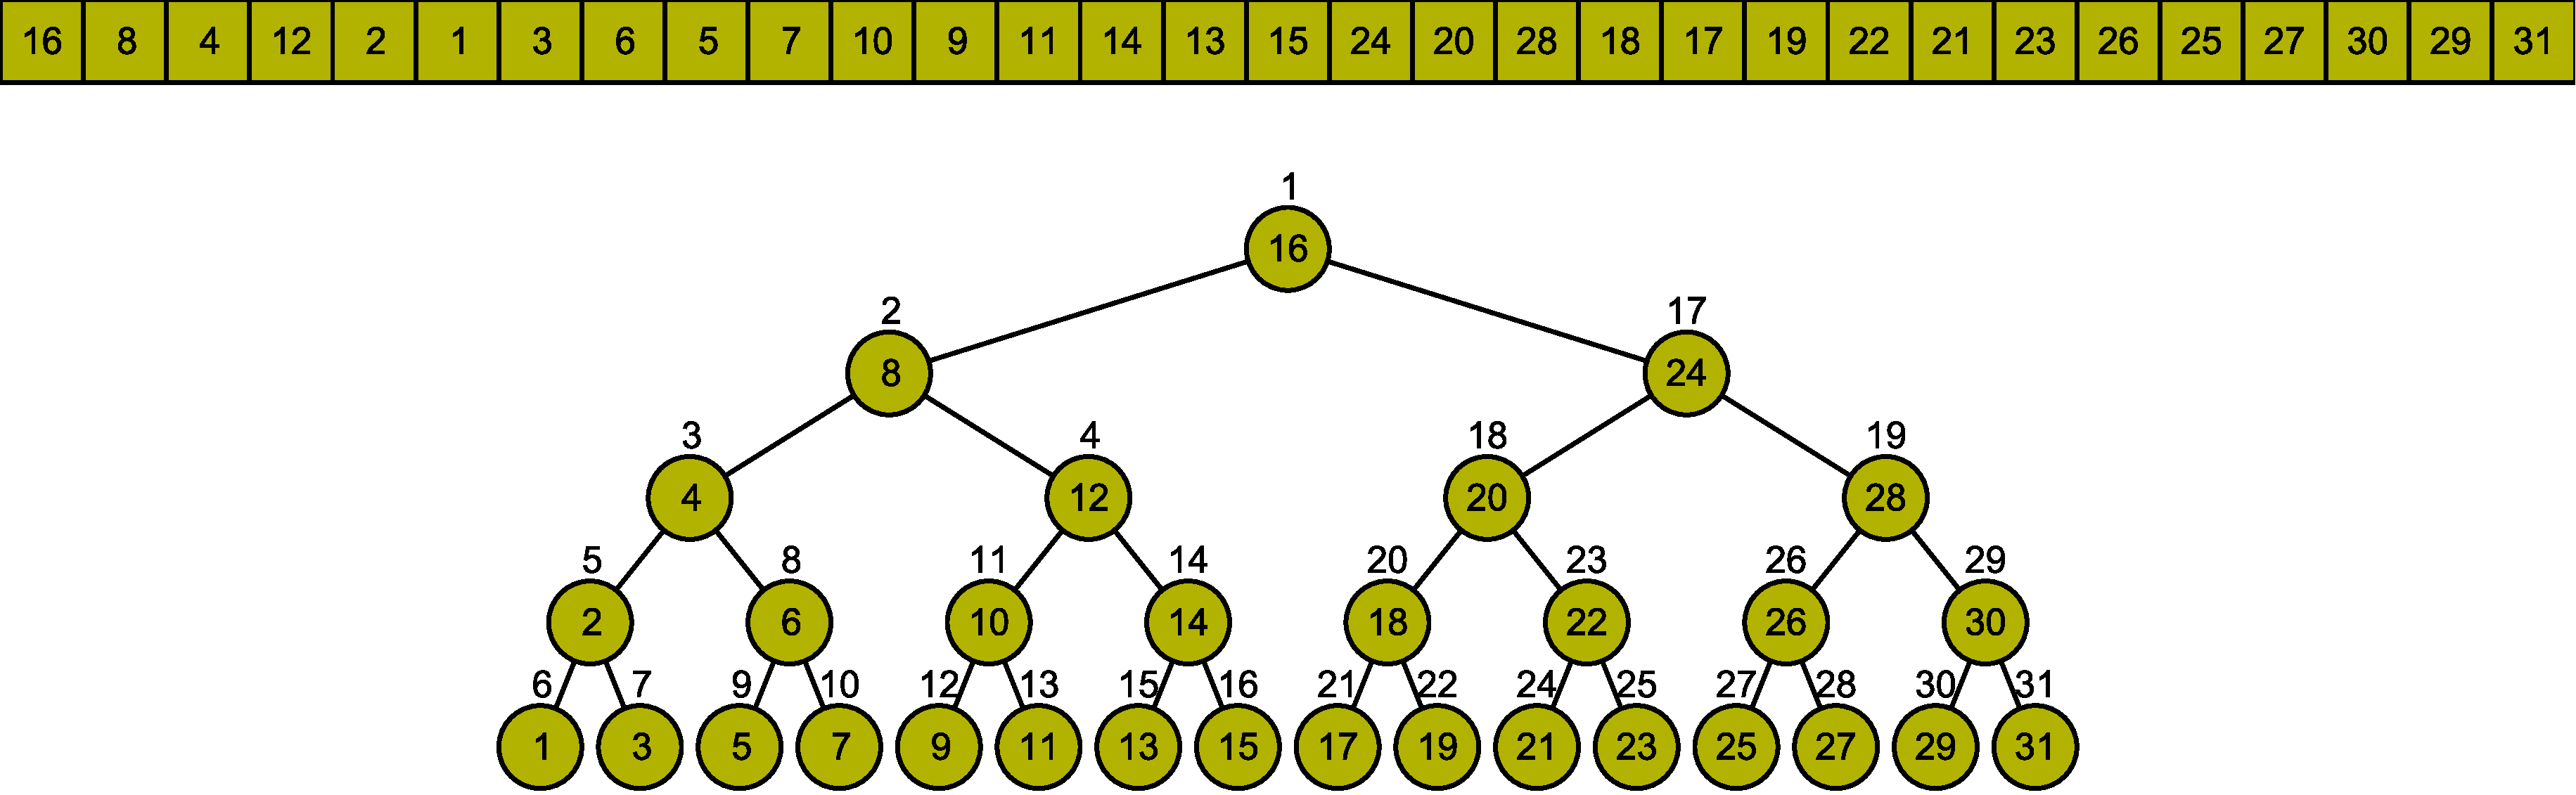
\includegraphics[width=\textwidth]{figures/screenshots/static_size_5.pdf}}
    \subtop[]{%
        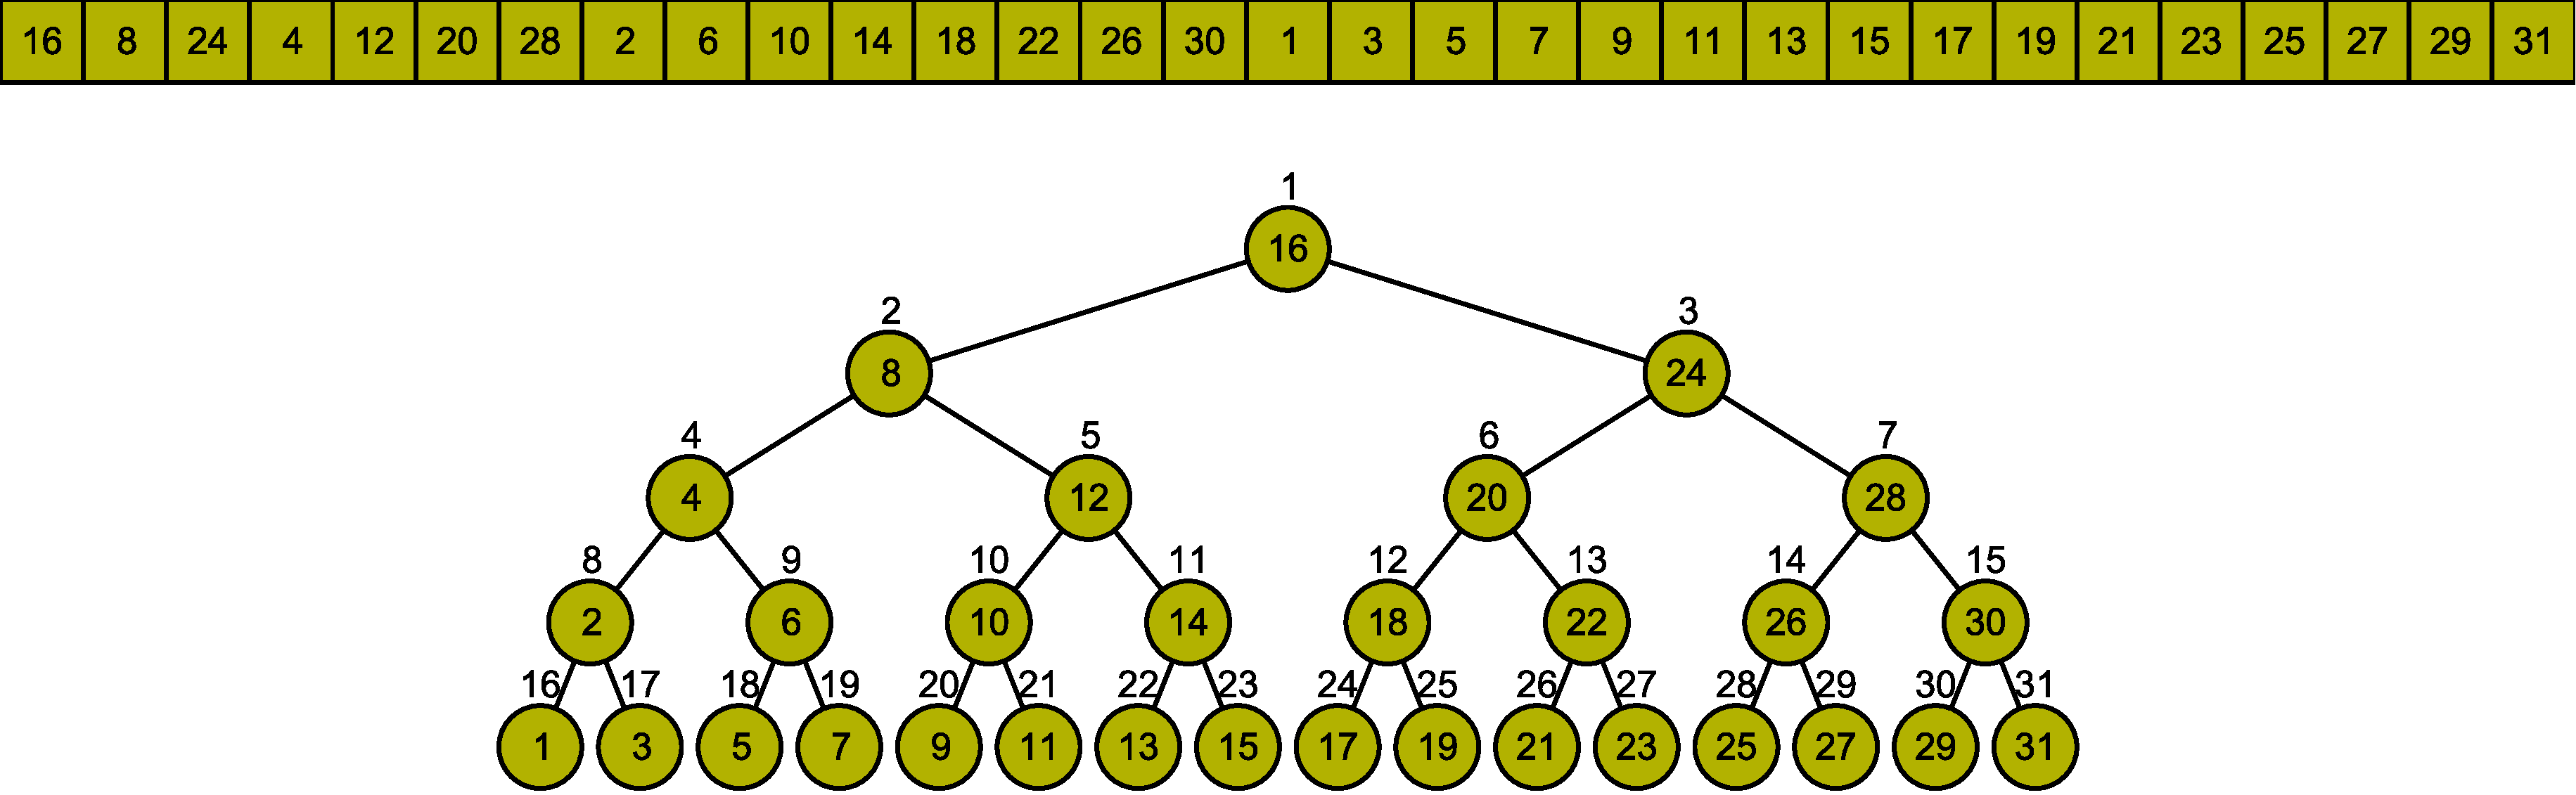
\includegraphics[width=\textwidth]{figures/screenshots/static_size_5_bfs.pdf}}
    \caption[Rozdiel medzi \emph{BFS} a \vEB usporiadaním]{Rozdiel medzi \emph{BFS} a \vEB usporiadaním na strome výšky~$5$. Kľúče zostávajú rovnaké, líšia sa však ich pozície v pamäti reprezentované malými číslami nad vrcholmi a poľom nad koreňom.}
    \label{fig:ss_static_order}
\end{figure}

\subsection{Simulácia \cache}
Porovnanie týchto dvoch usporiadaní je rozšírené o simuláciu \cache. Užívateľ si môže zvoliť parametre cache - počet vrcholov $B$, ktoré sa zmestia do jedného bloku a počet blokov $\frac{M}{B}$ v \cache. Tiež je možné \cache kedykoľvek vyprázdniť -- odstrániť z nej všetky načítané bloky. Simulácia na výmenu stránok používa stratégiu \emph{FIFO}, ktorá je popísaná v časti \ref{sec:memmng}.

Táto simulácia zároveň počíta počet prístupov k vrcholom pri vyhľadávaní a počet presunutých blokov do \cache. V najhoršom prípade by tieto dve čísla boli rovnaké (ak treba každý vrchol načítať osobitne) avšak pri \cache s blokmi veľkosti $B > 1$ a s \vEB usporiadaním dochádza k podstatnému zlepšeniu - ušetreniu počtu presunutých blokov.

To môžeme vidieť na jednoduchom príklade, kedy v strome výšky $5$ postupne vyhľadáme všetkých $16$ kľúčov, ktoré sa nachádzajú v listoch tohto stromu. V oboch usporiadaniach bude počet prístupov rovnaký, avšak počet načítaní blokov z disku do \cache je v tomto príklade pri \emph{BFS} usporiadaní takmer dvakrát väčší ako pri \vEB usporiadaní. Obrázok \ref{fig:ss_cachesim_compare} ukazuje stav týchto štatistík po nájdení posledného listu.

\begin{figure}[h]
    \centering
    \subbottom[Strom v \emph{BFS} usporiadaní] {
        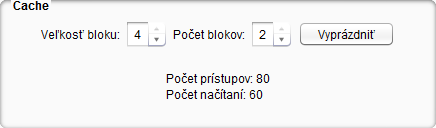
\includegraphics[width=6cm]{figures/screenshots/bmp_cache_panel_leaves_bfs}
    }
    \hspace{1cm}
    \subbottom[Strom vo \vEB usporiadaní] {
        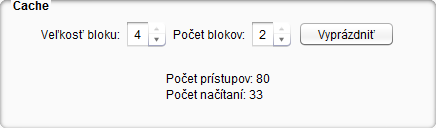
\includegraphics[width=6cm]{figures/screenshots/bmp_cache_panel_leaves_veb}
    }
    \caption[Porovnanie štatistík simulovanej \cache]{Porovnanie štatistík simulovanej \cache po prechode listov $1,3,\dotsc,31$ stromu výšky $5$. Parametre cache sú v oboch prípadoch rovnaké ($B=4$, $M=2B=8$), rozdiel je však v usporiadaní v pamäti.}
    \label{fig:ss_cachesim_compare}
\end{figure}

Ako vizualizácia prítomnosti v \cache slúži farba - vrcholy a položky poľa obsahujúce kľúče majú svetlejšiu farbu pozadia v prípade, že je daný blok v \cache a tmavšiu ak je mimo. V strome je vďaka tomu ľahko vidieť, ktorá časť je načítaná a je možné ňou prechádzať bez ďalších presunov. V prípade \vEB usporiadanie pôjde prevažne o časť podstromu aktuálne porovnávaného vrcholu, avšak pri klasickom usporiadaní to budú práve vrcholy mimo tohto podstromu, o ktorých už vieme, že nie sú pri vyhľadávaní potrebné.

\begin{figure}
    \centering
    \subtop[Nultý krok]{%
        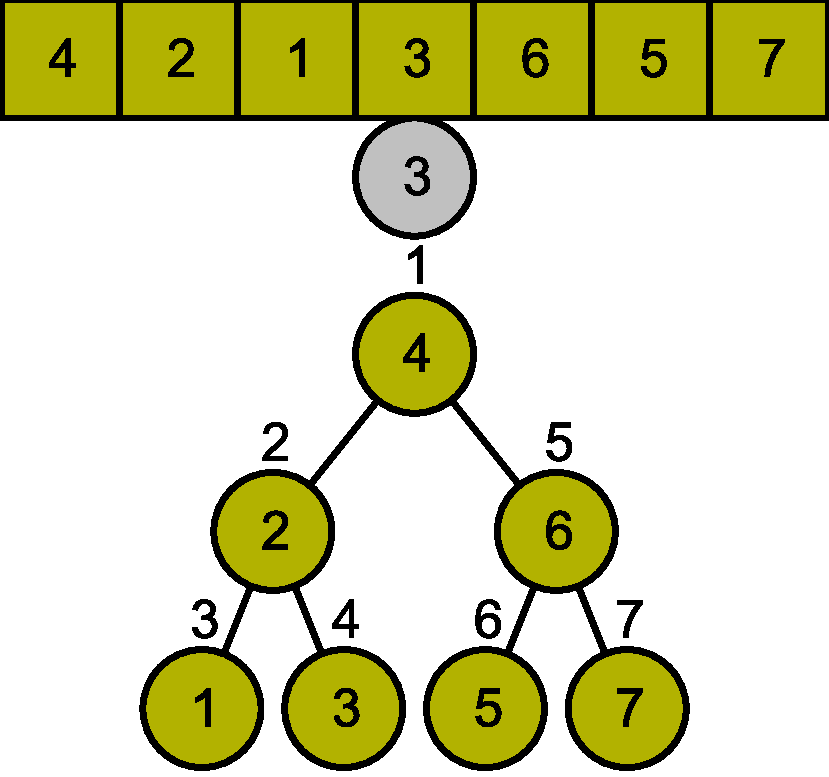
\includegraphics[width=0.25\textwidth]{figures/screenshots/cachesim_step1.pdf}}
    \hspace{1cm}
    \subtop[Prvý krok]{%
        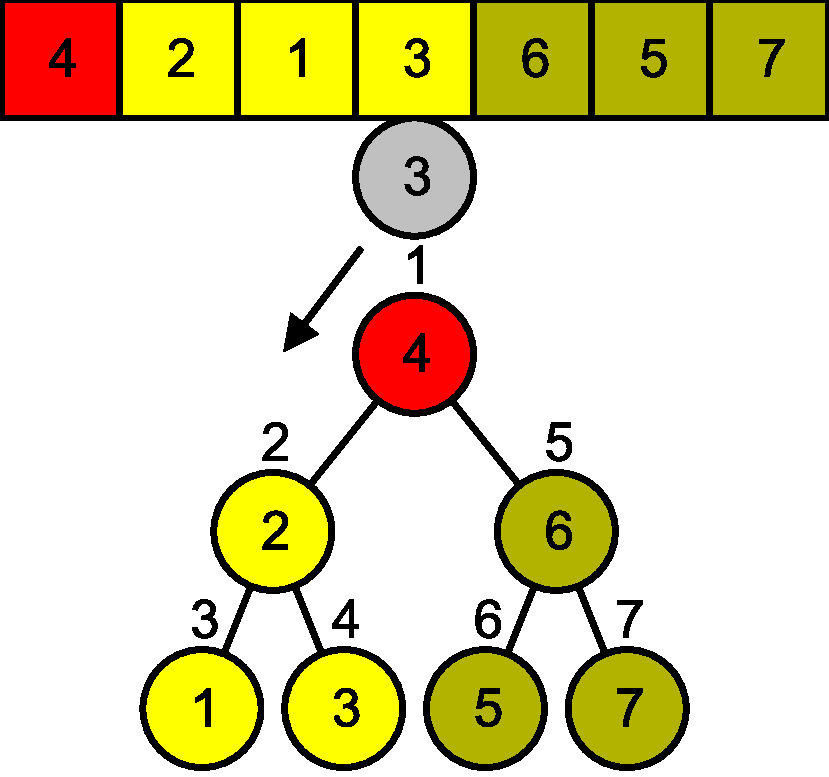
\includegraphics[width=0.25\textwidth]{figures/screenshots/cachesim_step2.pdf}}
    \hspace{1cm}
    \subtop[Druhý krok]{%
        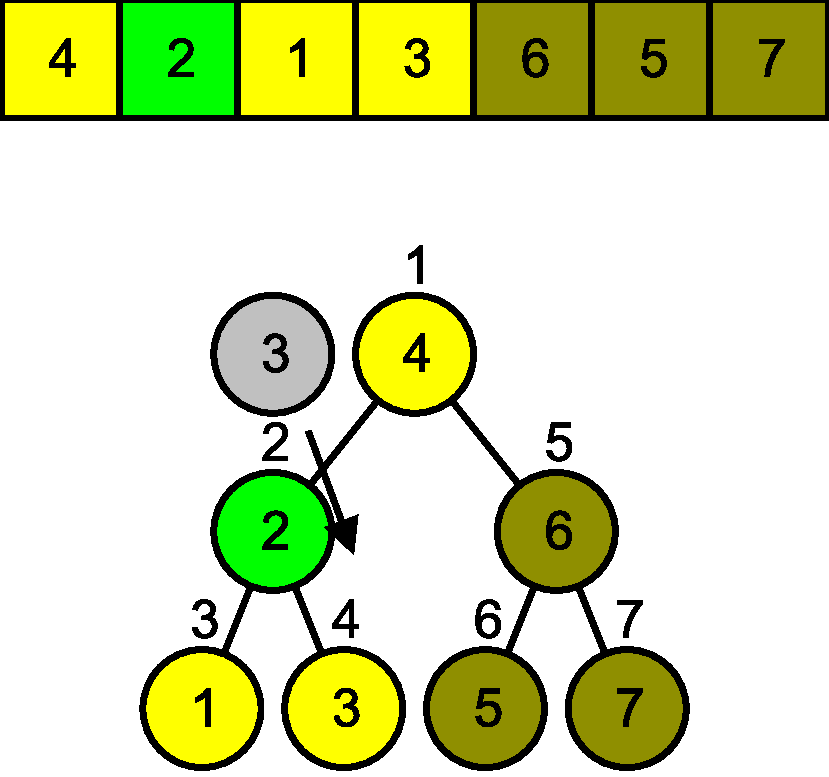
\includegraphics[width=0.25\textwidth]{figures/screenshots/cachesim_step3.pdf}}
    \caption[Simulácia \cache počas vyhľadávania kľúča]{Simulácia \cache počas vyhľadávania kľúča $3$. Pred prvým prístupom je cache prázdna. V prvok kroku načítame koreň, ktorý je označený červenou farbou (\miss), keďže nebol v \cache. Spolu s ním sa v jednom bloku načítali ďalšie vrcholy, ktoré su označené svetlejšou farbou. V druhom kroku je vrchol s kľúčom $2$ označený zelenou farbou (\hit), keďže už bol do \cache načítaný v predchádzajúcom kroku.}
    \label{fig:ss_cachesim_colors}
\end{figure}

Pri krokovaní vyhľadávania je pri prístupe k vrcholu tiež použitá zelená alebo červená farba na jeho dočasné zafarbenie (podobne ako v časti \ref{sec:memaccess_patterns}) podľa toho, či sa v danom momente v \cache nachádzal (\hit) alebo nie (\miss). Ukážka tohto zafarbovania je na obrázku \ref{fig:ss_cachesim_colors}.

\section{Usporiadané pole}
Ďalšou implementovanou vizualizáciou je usporiadané pole (obrázok \ref{fig:ss_of_overview}), ktoré bolo popísané v časti \ref{sec:orderedfile}. Bloky, na ktoré je toto pole imaginárne rozdelené sú znázornené tým, že sú od seba oddelené medzerou. Taktiež sa zobrazuje imaginárny strom nad týmito blokmi, ktorým sa pri vkladaní prechádza. Hodnoty vo vrcholoch reprezentujú hustotu (v percentách) intervalu v príslušnom podstrome. Farby (zelená alebo červená) vrcholov indikujú, či sa hustota daného vrcholu nachádza v hraniciach.

\begin{figure}
    \centering
    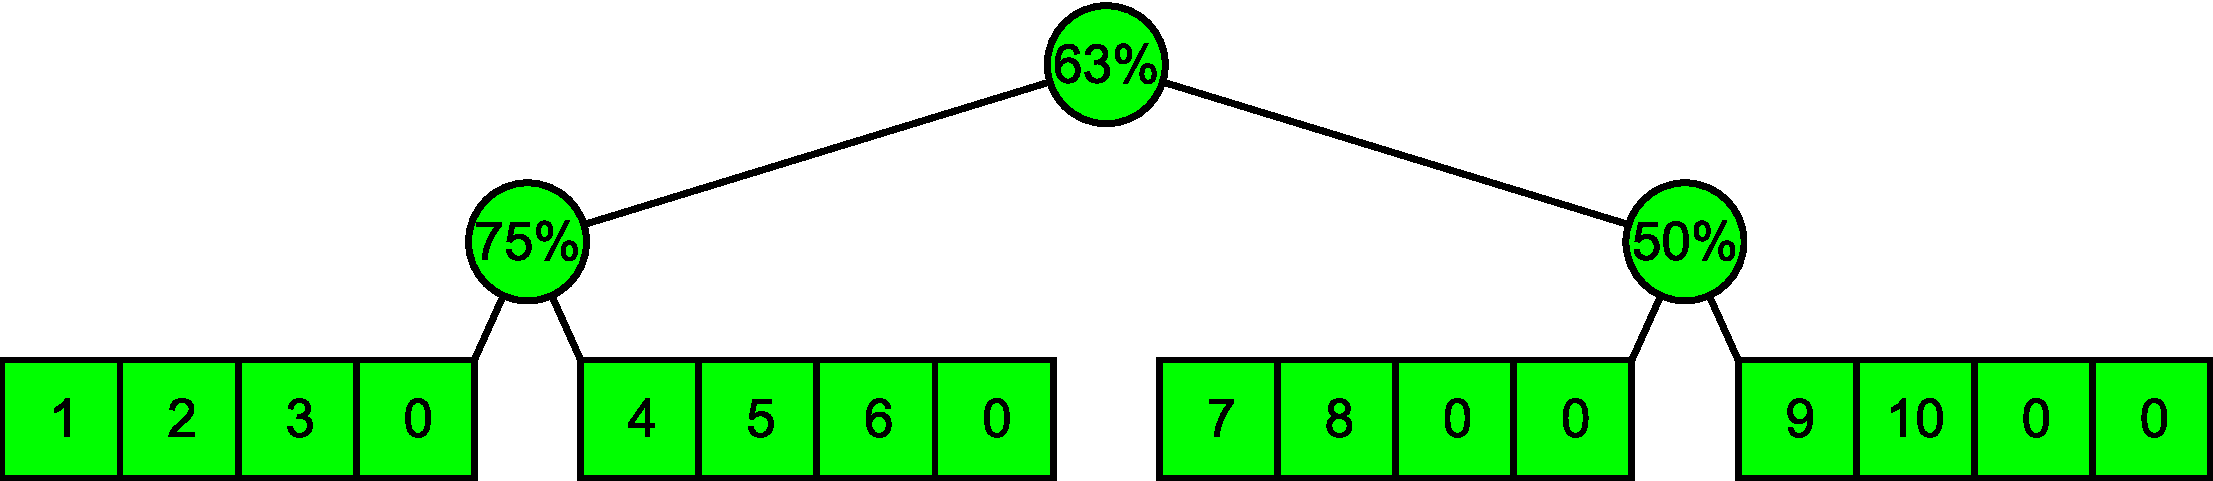
\includegraphics[width=0.8\textwidth]{figures/screenshots/of_overview_3.pdf}
    \caption[Usporiadané pole]{Usporiadané pole obsahujúce hodnoty $1$ až $10$. Všetky vrcholu majú hustotu v hraniach hustoty. Hodnoty $0$ reprezentujú prázdne pozície.}
    \label{fig:ss_of_overview}
\end{figure}

Táto vizualizácia podporuje vkladanie hodnoty na ľubovolnú pozíciu v poli. V prípade, že sa pole preplní, automaticky sa vytvorí nové, dvojnásobne väčšie. Po vložení hodnoty je tiež vyznačený interval, ktorý sa zmenil.

\section{Dynamický strom}
Vizualizácia dynamického stromu (časť \ref{sec:dynamic-obliv}) vznikla spojením predchádzajúcich dvoch vizualizácií (obrázok \ref{fig:ss_cobtree}). Horná časť je statický strom vo \vEB usporiadaní (obrázok \ref{fig:ss_static_sizes}), dolná je usporiadané pole (obrázok \ref{fig:ss_of_overview}), pričom strom hustôt je tu preklopený nadol, aby sa neprekrýval so statickým stromom. Hrany medzi nimi spájajú listy stromu s prvkami usporiadaného pola. 

\begin{figure}
    \centering
    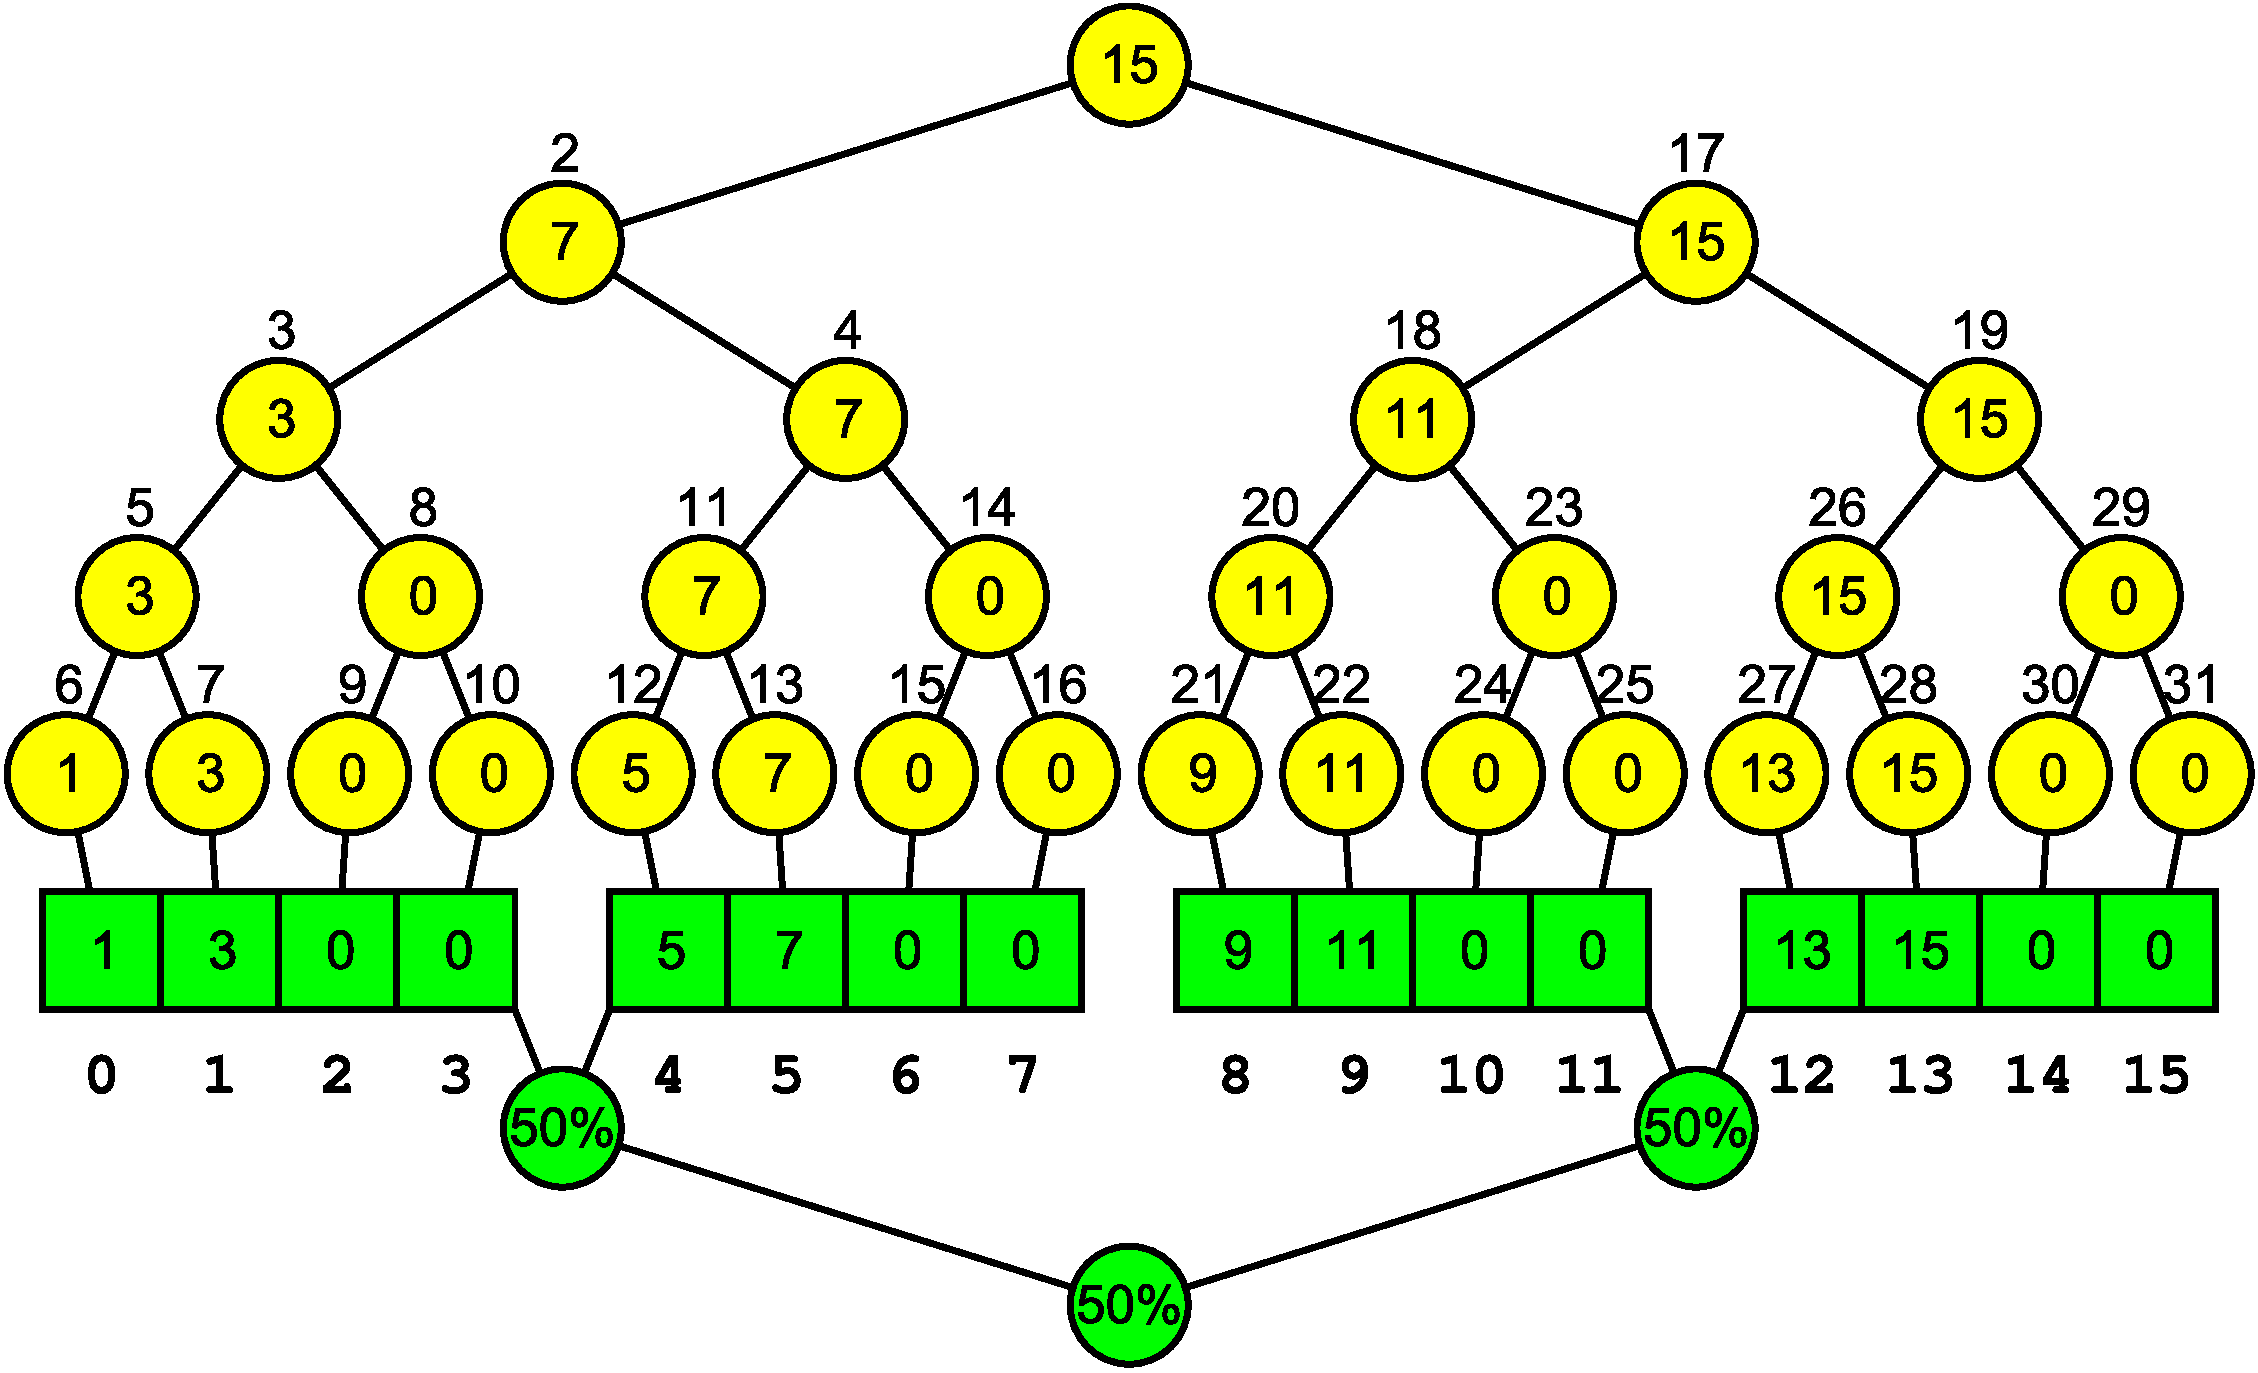
\includegraphics[width=0.8\textwidth]{figures/screenshots/cobtree_overview.pdf}
    \caption[Vizualizácia dynamického \obliv B-stromu]{Vizualizácia dynamického \obliv B-stromu.}
    \label{fig:ss_cobtree}
\end{figure}

V tomto strome je možné vyhľadávať a vkladať do neho nové kľúče. Pri vkladaní prebehne najskôr vloženie do usporiadaného poľa rovnako, ako pri jeho samostatnej vizualizácii. Následne sa aktualizujú kľúče statického stromu. V prípade zdvojnásobenia veľkosti statického poľa sa vytvorí nový, väčší statický strom.


\section{Implementácia}
\todo[inline]{?}

%Visualization
%- intro
%- existing - none?
%- algvis history
%- implementation details
%  - cache simulation
%- list of structures
%  - static tree
%    - intro
%    - array order
%    - cache simulation
%    - order switching
%  - ordered file
%    - intro
%    - insert
%  - cobtree
%    - intro
%    - layout
%    - find
%    - insert
%- testovanie?
